%Definição e proposta de metodologias a usar, com vista à consecução dos objetivos da Dissertação
%Resultados esperados e eventuais resultados preliminares
%Planificação e calendarização do trabalho a desenvolver na Dissertação

%SoC
\subsection{System-on-Chip}
A System-on-Chip (SoC) is an integrated circuit that combines components of an electronic system. These components usually include a Central Processing Unit (CPU), memory interfaces, on-chip input/output devices, input/output interfaces, and secondary storage interfaces.\\
Putting many elements of a computer system on a single piece of silicon has some advantages, such as low power requirements, reduced cost, increased performance, and reduced physical size.
\vspace*{-0.05cm}
\subsection{IOb-SoC}
%iob-soc (%components, fpga resources, repository, accelerators)
The IOb-SoC is a System-on-Chip template, comprising an open-source RISC-V processor, which users can modify, simulate and implement in ASICs and FPGAs.
This SoC, provided by \textit{IObundle, Lda}, supports stand-alone and boot-loading modes. It also allows an internal RAM or an external DDR controller via an L1/L2 cache system. 

Figure \ref{fig:iob} shows the IOb-SoC high-level block diagram.

\vspace{0.1cm}

\begin{figure}[H]
\centerline{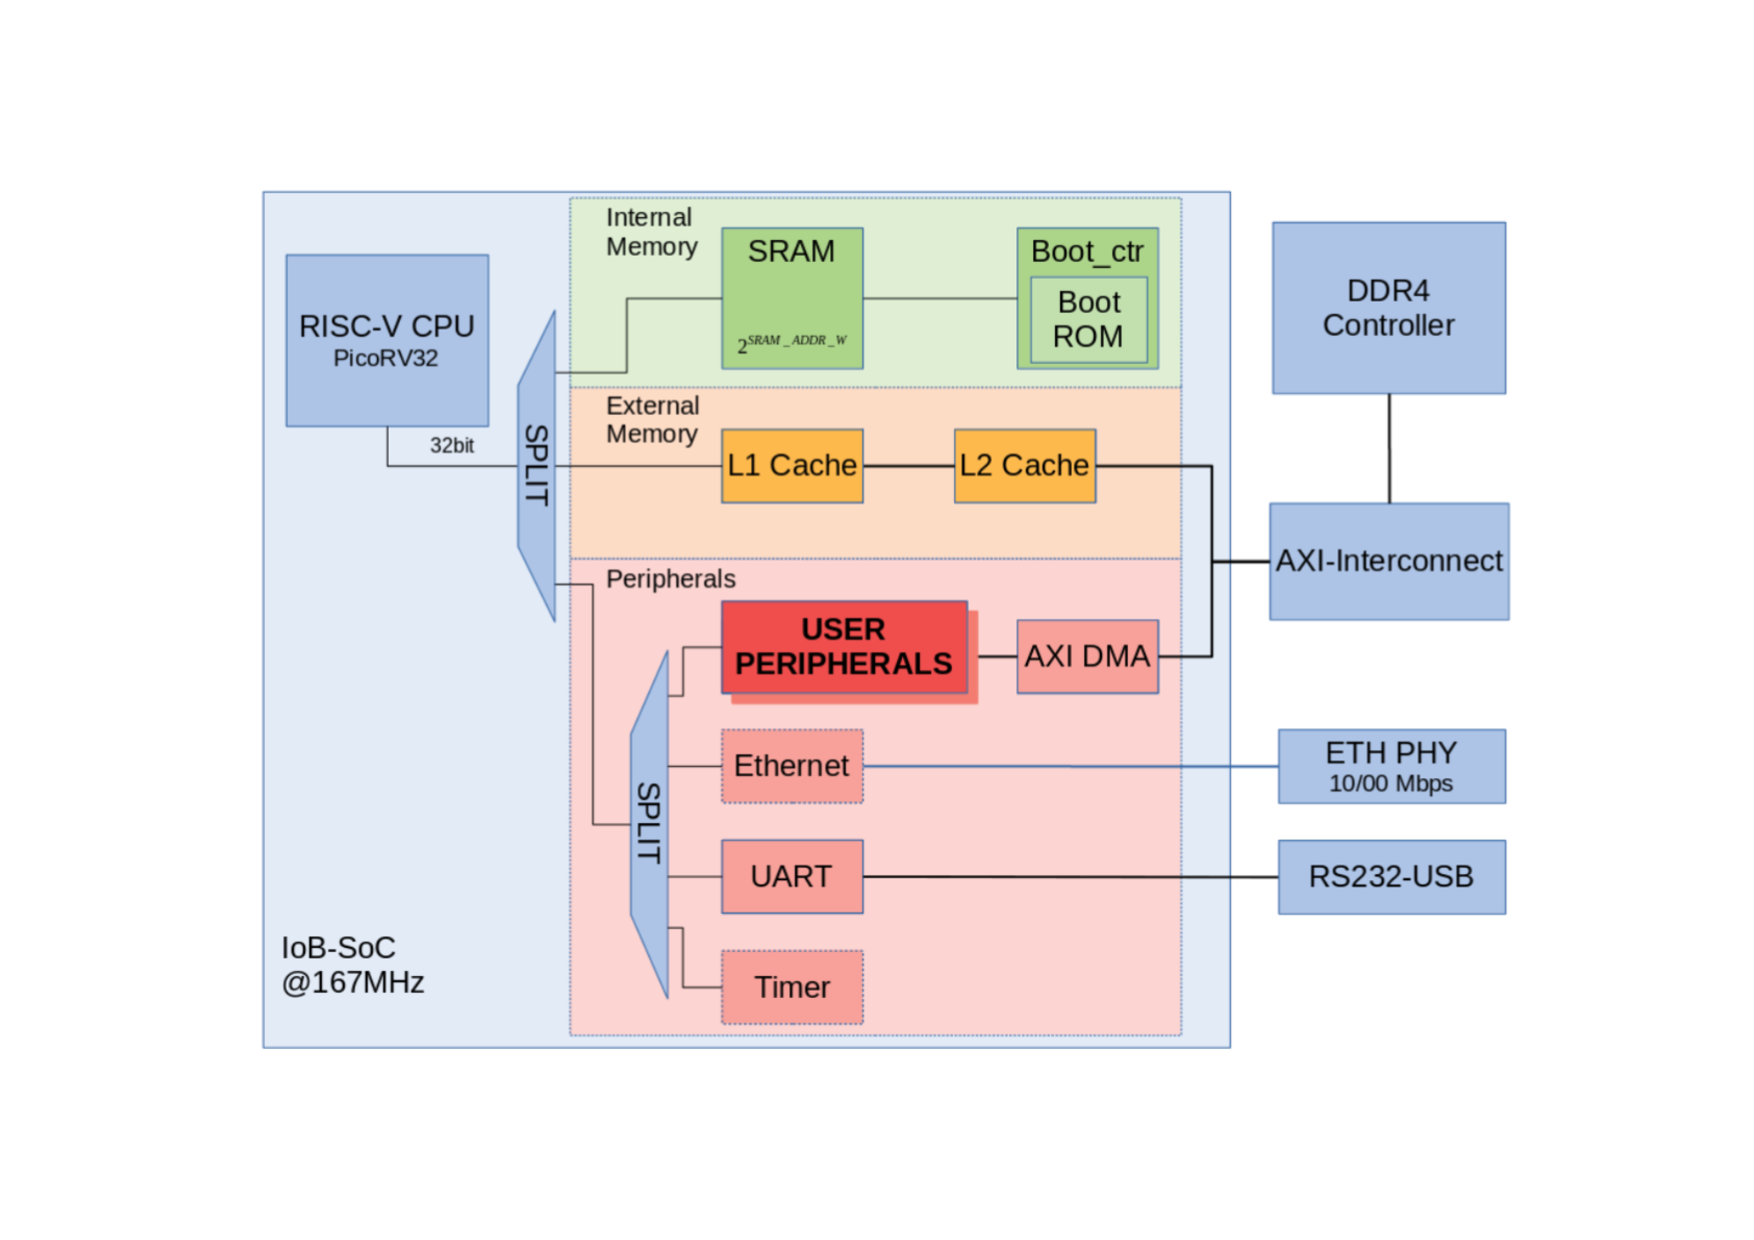
\includegraphics[width=0.85\linewidth]{iob-soc.pdf}}
\caption{IOb-SoC high-level block diagram.}
\label{fig:iob}
\end{figure}

\subsubsection{IOb-SoC Components}
Starting with the \textbf{CPU}, the IOb-SoC uses a PicoRV32 CPU core, an open-source 32-bit processor that implements the RV32IMC instruction set, with an operating frequency of 167MHz.

As \textbf{Memory} subsystem, this SoC includes three main components. The Boot Read-Only Memory \textbf{Boot ROM} is a ROM used for booting the system. The Static Random Access Memory \textbf{SRAM} is an internal memory that allows the system to run the program or the bootloader without the need for external memory. The \textbf{Cache} is an optional component that stores data from the external Double Data Rate (DDR) memory.

The communication between the CPU and the system’s components (master and slaves) occurs through two buses. The \textbf{Memory bus} allows the CPU to communicate with the memory subsystem, while the \textbf{Peripheral bus} allows the CPU to communicate with system peripherals.

In addition, the \textbf{IOb-Interconnect} component is a bus switch responsible for the valid-ready handshake protocol between the CPU and all the peripherals. Based on the peripheral prefix from the address bus, this component selects which peripheral-specific bus connects to the CPU bus. \\
The \textbf{IOb-Interconnect} multiplexes or demultiplexes, depending on the direction, the CPU bus signals (\textit{valid}, \textit{ready} and \textit{rdata}). By doing so, the component creates enough signals to ensure that there is one of each signal for each of the peripherals. Optionally, two peripherals connected to the peripheral bus can communicate directly without CPU intervention, allowing for faster data transfers between peripherals.

There is also a \textbf{Native to AXI adapter}, which allows communication between peripherals and memory controllers that use the AXI4 protocol. Since the CPU only contains the native bus, the IOb-SoC uses this component to convert the signals from one bus to the other, with each peripheral that uses the AXI4-Lite port containing one \textbf{Native to AXI adapter}.

Finally, The Universal Asynchronous Receiver-Transmitter (\textbf{\textbf{UART}}) peripheral allows the SoC to communicate with external systems, through the RS-232 serial communication protocol. 

\subsubsection{IOb-SoC Deliverables and FPGA Resources}
As deliverables, the IOb-SoC includes Hardware Description Language (HDL) source code, software C source code, simulation testbench, implementation constraints for map, place, and route, demo files, and user documentation for system integration.

Tables~\ref{tab:resorucesxilinx} and~\ref{tab:resorucescyclone} show the implementation resources used for \textit{Xilinx Kintex Ultrascale Devices} and \textit{Intel Cyclone V Devices}, respectively, according to the product brief.

\vspace{0.8cm}

\begin{table}[H]
\parbox{.45\linewidth}{
\centering
\begin{tabular}{|c|c|c|}
        \hline
         \textbf{Resource} & \textbf{Usage}  \\
         \hline
         LUTs & 1869 \\
         \hline
         Registers & 1029 \\
         \hline
         DSPs & 4 \\
         \hline
         BRAM & 5 \\
         \hline
         PIN & 6 \\
         \hline
\end{tabular}
\caption{Implementation resources for Xilinx Kintex
Ultrascale Devices.}
\label{tab:resorucesxilinx}
}
\hfill
\parbox{.45\linewidth}{
\centering
\begin{tabular}{|c|c|c|}
        \hline
         \textbf{Resource} & \textbf{Usage}  \\
         \hline
         ALM & 1335 \\
         \hline
         FF & 1177 \\
         \hline
         DSP & 3 \\
         \hline
         BRAM blocks & 22 \\
         \hline
         BRAM bits & 165,888 \\
         \hline
         PIN & 6 \\
         \hline
\end{tabular}
\caption{Implementation resources for Intel Cyclone
V Devices.}
\label{tab:resorucescyclone}
}
\end{table}

%If the external memory interface is selected, an instruction L1 cache, a data L1 cache, and a shared L2 cache are added to the system. The L2 cache communicates with a 3rd party memory controller IP (typically a DDR controller) using an AXI4 master bus.

\subsubsection{IOb-SoC Repository}

%peripherals
%simulators and FPGA
The IOb-SoC Repository is a \textit{GitHub} repository that allows the user to modify the system components easily. It contains specific directories and segments (Tool Command Language (TCL), Verilog, Makefile, etc), with the list below describing the main items.

\textbf{document/} This directory supports all the documentation, from LaTeX code and scripts to generated pdfs, like the guide and product brief.

\textbf{hardware/} This directory supports the hardware layer, containing multiple subdirectories.

\hspace{0.5cm} – \textbf{hardware.mk} This makefile contains targets, dependencies, and rules related to hardware.

\hspace{0.5cm} – \textbf{fpga/} This directory contains scripts to synthesize and run the system in FPGAs.

\hspace{1.2cm}\textbf{fpga.mk} This makefile contains targets, dependencies, and rules related to FPGAs.

\hspace{0.5cm} – \textbf{simulation/} This directory contains scripts to run RTL simulation in simulators.

\hspace{1.2cm}\textbf{simulation.mk} This makefile contains targets, dependencies, and rules related to simulators.

\hspace{0.5cm}– \textbf{src/} This directory contains Verilog scripts related to the system’s components.

\textbf{software/} This directory supports the software layer, containing multiple subdirectories.

\hspace{0.5cm}– \textbf{software.mk} This makefile contains targets, dependencies, and rules related to software.

\hspace{0.5cm}– \textbf{firmware/} This directory contains the software to run in the system, after initialization.

\hspace{0.5cm}– \textbf{bootloader/} This directory contains the bootable software for the system.

\hspace{0.5cm}– \textbf{pc-emul/} This directory contains scripts to run the firmware on the computer.

\hspace{0.5cm}– \textbf{console/} This directory contains the software that allows interaction between computer and FPGA, via UART.

\textbf{submodules/} This directory contains all submodules and peripherals used in the system. While the peripherals are added to the peripheral bus, the submodules only represent components that are integrated into the system. 

\textbf{config.mk} This makefile contains targets, dependencies, and rules related to the SoC configuration, like the list of peripherals.

\subsection{ISO/SEC 11172-3: 1993 (E)}

The ISO/IEC 11172 is an international standard under the title \textit{Information technology - Coding of moving pictures and associated audio for digital storage media at up to about 1,5 Mbit/s}. This standard is divided into four parts (Systems, Video, Audio, and Compliance testing), with the Audio part being the relevant one for this work.

Focusing on the audio, the ISO/IEC 11172-3 specifies the coded representation of high-quality audio for storage media, and also the method for decoding high-quality audio signals. \\
Therefore, this part is intended for application to digital storage media. It provides a total continuous transfer rate of around 1.5Mbits/sec for both audio and video bitstreams, with sampling rates of 32kHz, 44.1kHz, and 48kHz.

\subsubsection{Audio encoder}

The audio encoder is responsible for processing the digital audio signal and producing the compressed bitstream for storage. 
The encoder algorithm is not standardized and may use various means of encoding, such as estimation of the auditory masking threshold, quantization, and scaling. However, the encoder output must be such that a decoder, conforming to the specifications of the coded audio bitstream, will produce audio suitable for the intended application.

%figure page v iso
Figure \ref{fig:encoder} illustrates the basic structure of an audio encoder. 

\begin{figure}[H]
\centerline{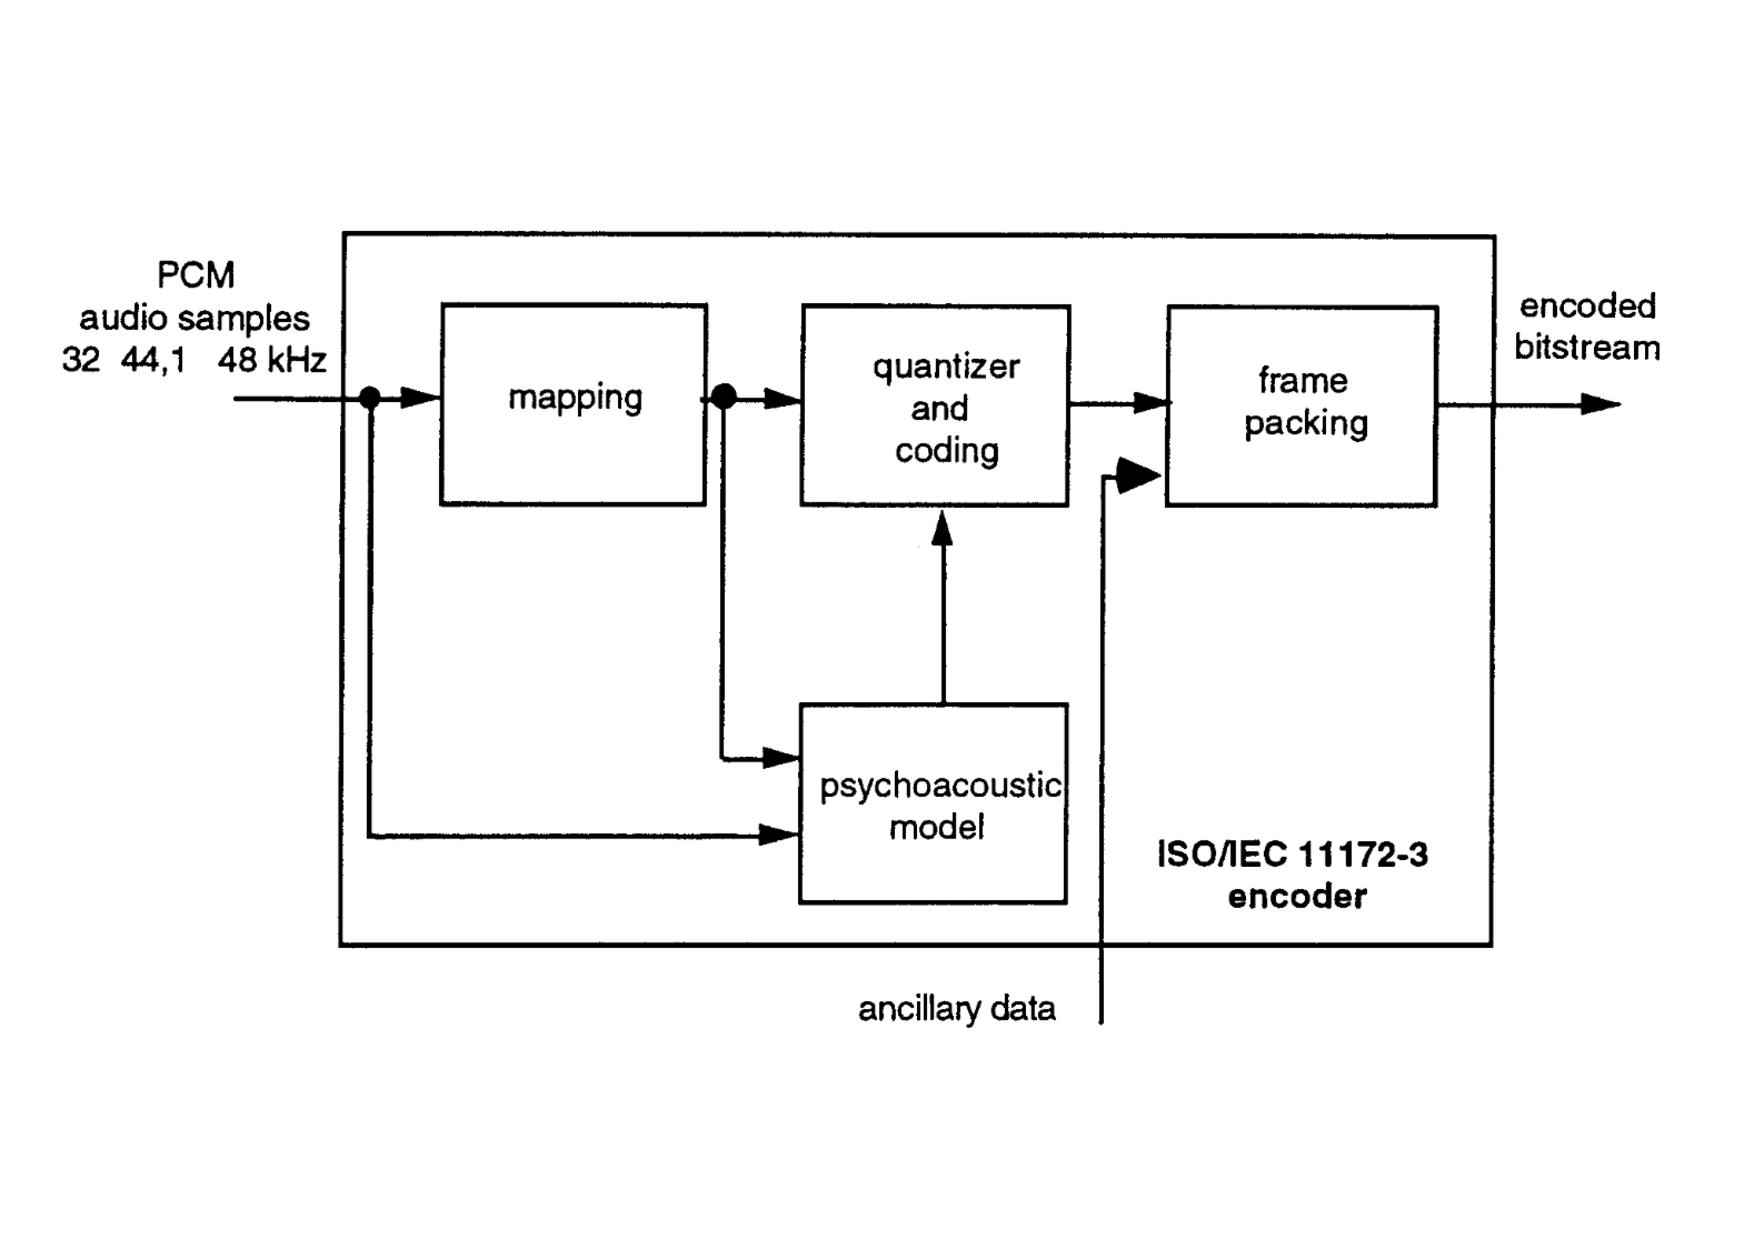
\includegraphics[width=0.85\linewidth]{encoder.pdf}}
\caption{Audio encoder basic structure.}
\label{fig:encoder}
\end{figure}

The encoding process contains four main blocks: \textit{mapping}, \textit{psychoacoustic model}, \textit{quantizer and coding}, and \textit{frame packing}.

First, the \textbf{mapping} block creates a filtered and subsampled representation of the input audio stream, usually called subband samples (for Layer II). At the same stage, the \textbf{psychoacoustic model} block creates a set of data to control the next block (\textit{quantizer and coding}). These control data depend on the coder implementation, with one possibility being the use of a masking threshold estimation.

Then, the \textbf{quantizer and coding} block creates a set of coding symbols from the mapped input samples, depending on the encoding system once again. 

Finally, the \textbf{frame packing} block assembles the actual bitstream from the output data of the previous blocks, adding information if necessary.

The encoding process supports four different modes: single channel, dual channel (two independent audio signals coded within one bitstream), stereo (left and right signals of a stereo pair coded within one bitstream), and Joint Stereo (with the stereo irrelevancy and redundancy exploited).

\subsubsection{Psychoacoustic encoder}

The ISO/IEC 11172-3 (MPEG-Audio) psychoacoustic algorithm contains four primary parts, as shown in figure \ref{fig:algorithm}: \textit{Filter Bank}, \textit{Psychoacoustic Model}, \textit{Bit or Noise Allocation} and \textit{Bitstream Formatting}.

%figure page 66 iso
\begin{figure}[H]
\centerline{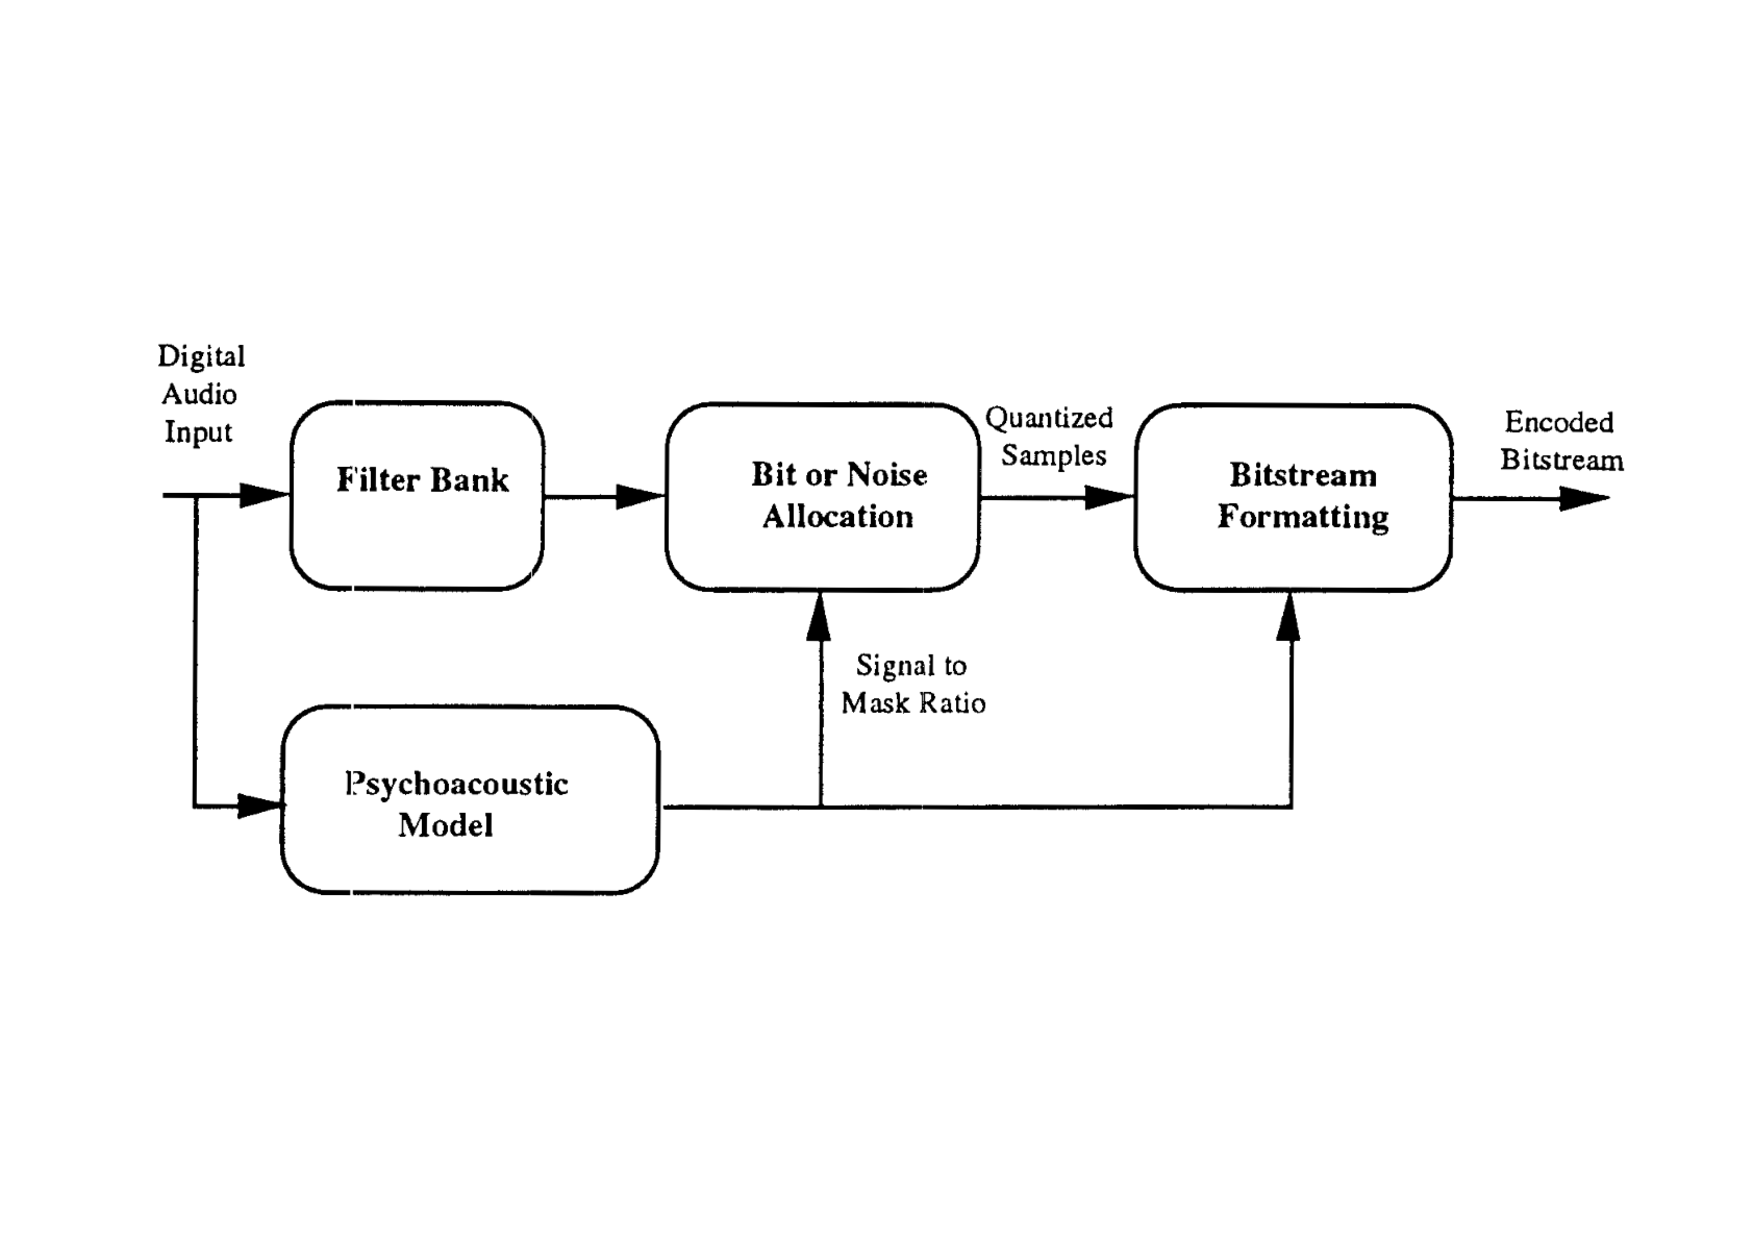
\includegraphics[width=0.85\linewidth]{iso-encoder.pdf}}
\caption{ISO/IEC 11172-3 encoder block diagram.}
\label{fig:algorithm}
\end{figure}

The \textbf{Filter Bank} does a time-to-frequency mapping, being one of two types. It can be a polyphase filter bank or a hybrid polyphase/MDCT filter bank, with each delivering a specific mapping in time and frequency.
These filterbanks are critically sampled, having the same number of samples in both analyzed and time domains, and provide the primary frequency separation for the encoder, with quantized output samples. \\
In layer II, a filter bank with 32 subbands is used. In each subband, 12 or 36 samples are grouped for processing.

The \textbf{Psychoacoustic Model} calculates a just noticeable noise level for each band in the filter bank. This noise level is used in the \textit{Bit or Noise Allocation} part to determine the actual quantizers and quantizer levels. 
The final output of the model is a signal-to-mask ratio (SMR) for each band (Layer II).
%annex D  (MOdel 1 Layer II)

The \textbf{Bit or Noise Allocation} takes both the output samples from the \textit{Filter Bank} and the SMR from the \textit{Psychoacoustic Model} and adjusts the bit allocation, to meet the bitrate and masking requirements. At low bitrates, these methods attempt to spend bits in a way that is inoffensive when they cannot meet the psychoacoustic demand at the required bitrate.\\
In Layer II, this method is a bit allocation process, where several bits are assigned to each sample (or group of samples) in each subband.

The \textbf{Bitstream Formatting} takes the quantized filterbank outputs, together with the bit allocation and other required side information, and encodes and formats all that information in an efficient way.\\
In Layer II, a fixed Pulse code modulation (PCM) code is used for each subband sample, with the exception that quantized samples may be grouped.

%figure page 79 iso
Figure \ref{fig:flow-encoder} shows a more detailed Layer II Encoder flow chart.

\begin{figure}[H]
\centerline{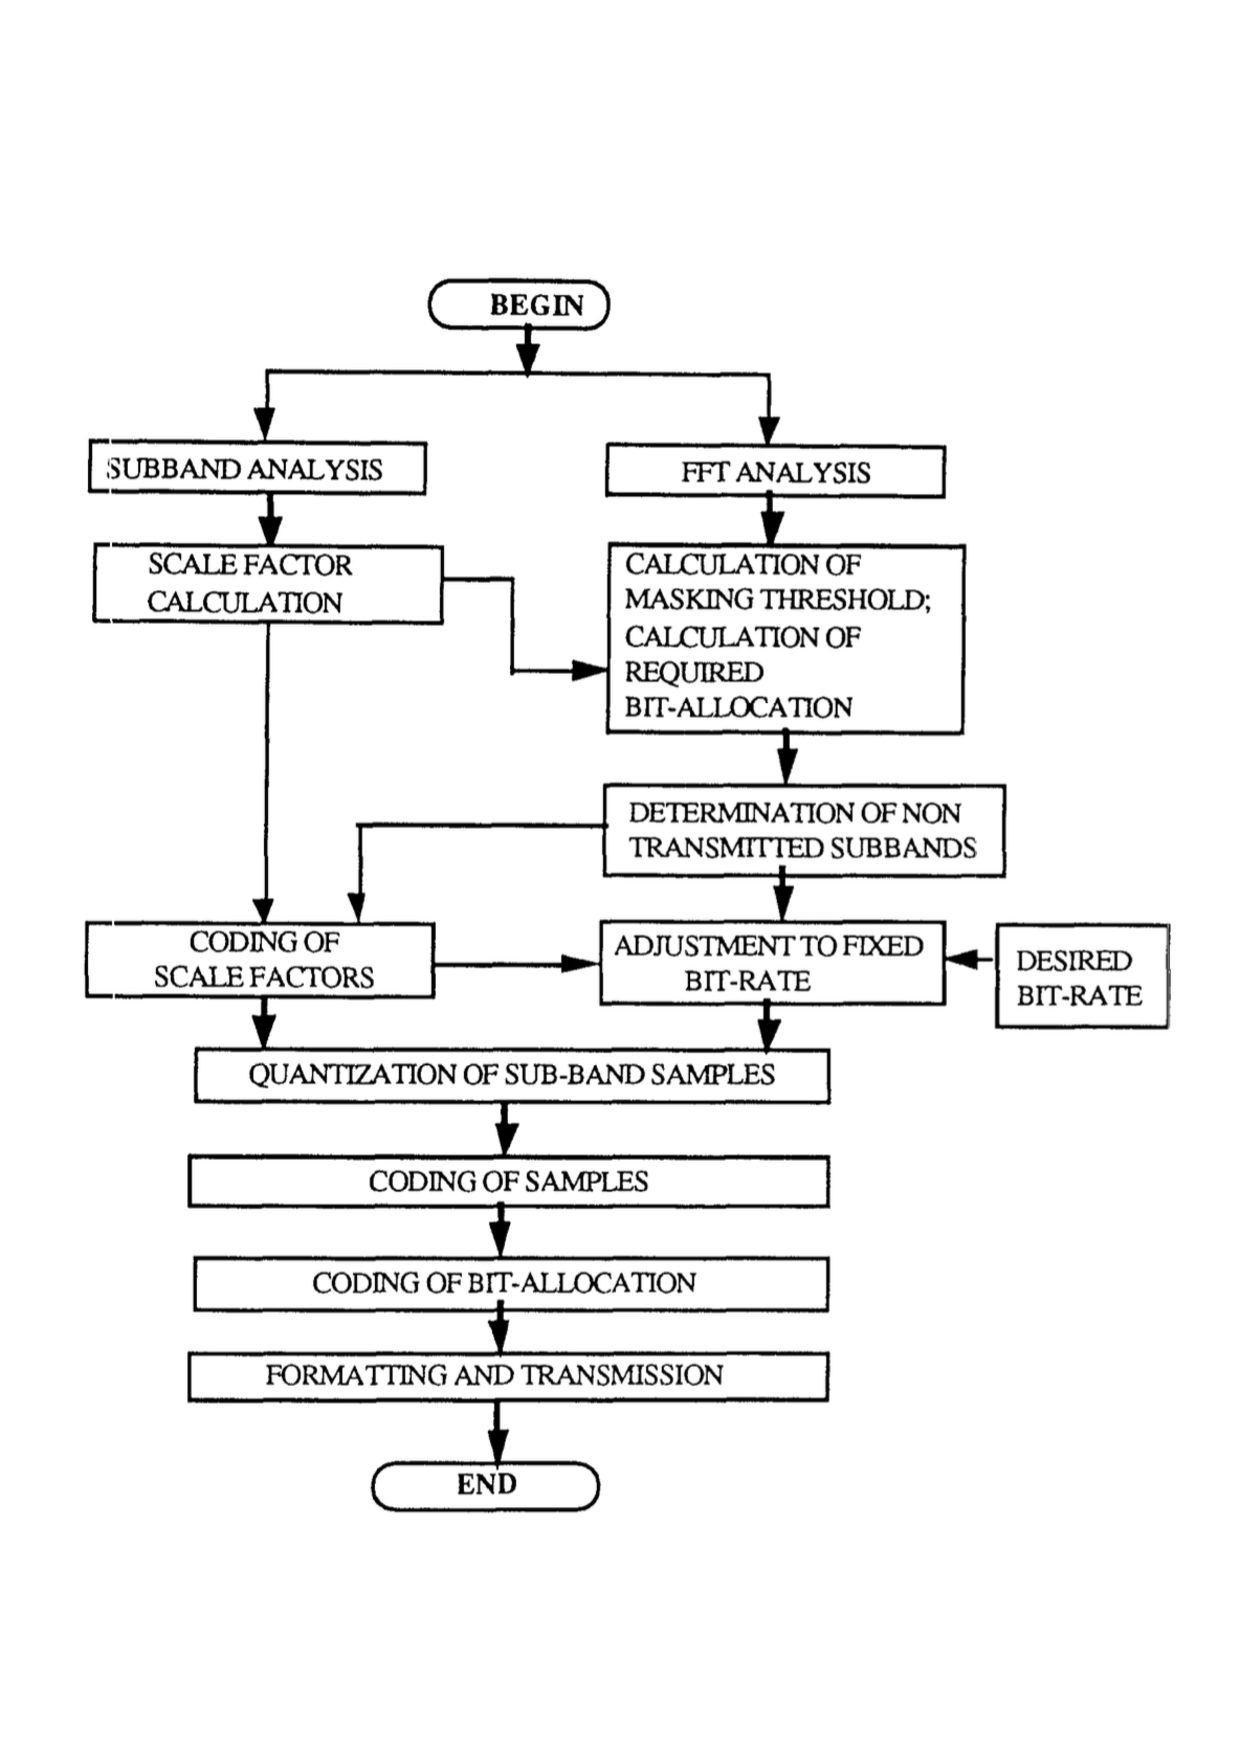
\includegraphics[width=0.70\linewidth]{flow-encoder.pdf}}
\caption{Layer II encoder flow chart.}
\label{fig:flow-encoder}
\end{figure}

\subsection{Hardware/Software}

The \textit{TwoLAME} software will be ported to IOb-SoC's CPU (PicoRV32). However, when encoding at the sampling frequency, the system may not finish execution in real-time. If this is the case, a peripheral will be developed to accelerate the process bottlenecks.

In addition, \textit{TwoLAME} uses floating-point arithmetic (FP)~\cite{floatingpoint}, which can make the hardware implementation quite large. Therefore, developing the peripheral with fixed-point arithmetic~\cite{fixedpoint} would be plausible.
In this case, the VexRiscv (RV32IM) CPU could be used, since it includes a floating-point unit (FPU)~\cite{fpu}. To allow transferring data between the CPU and the peripheral (accelerator), two hardware converters (from floating-point/fixed-point to fixed-point/floating-point) would also be required.